\documentclass[12pt, letterpaper]{article}
\usepackage[utf8]{inputenc}
\usepackage{amsmath}
\usepackage{parskip}

\usepackage{graphicx}
\graphicspath{{../images/}}

\usepackage{hyperref}
\hypersetup{
    colorlinks=true,
    urlcolor=blue,
    linkcolor=blue,
    citecolor=blue,
    filecolor=blue,
}
\urlstyle{same}

\title{Notes to Feature Engineering}
\author{}
\date{}


\begin{document}

\maketitle

Extending the original feature set with new informative covariates which are created from (combinations of) existing variables is a central aspect of every data analysis.
Besided many numeric features the Airbnb data contains \emph{images} as well as \emph{reviews} in raw text form.
These data types in particular require some preprocessing steps which will be the focus of this section.

In addition, some basic data cleaning steps were necessary.
These mostly consisted of converting data types, splitting text-based variables into more convenient numeric or boolean features and aggregating rare categories of categorical variables into one larger \emph{Other} group to stabilize estimation.


\section{Image Processing and Modeling}

Besides the metric and text-based features the Airbnb Data contains \emph{images} of the listed apartments as well as of the corresponding hosts.
This section describes how we used these images (while focusing on the apartment pictures) for the purpose of price prediction.

The main idea was to build a Convolutional Neural Network that predicts the price solely based on the image content itself and add these predictions as well as the number of available images for each listing to the main feature set.
Since there exist multiple images per apartment, the predictions were averaged afterwards within each group to obtain an output array of equal length to all remaining features.

\subsection{Webscraping}

In the first step, the raw image links provided by the data set had to converted to an image format that the neural network is able to work with.

Therefore we first used the \texttt{requests} library to get the \texttt{HTML} Source Code of each listing's website.
Next, the \texttt{beautifulsoup} library served as a convenient HTML parser to find and extract all embedded weblinks that lead to images located on the front page of the listings website.
With this strategy we could extract the first $5$ images for each apartment (if $5$ or more were available) that could be directly accessed from the front page source code.

Finally, we used the \texttt{requests} module again in combination with the \texttt{pillow} package to decode the source content of all image adresses into two dimensional images.


\subsection{Preprocessing}

Before feeding these two dimensional images into the model, we performed some further preprocessing steps.

One very common technique when dealing with images is \emph{Data Augmentation}.
In contrast to classification tasks however, where Data Augmentation is used to expand the training set and improve simultaneously generalization, this approach is not immediately transferable to a regression context since we have to guarantee that the label (i.e. the price) remains unchanged for each image transformation.
Thus, we decided against standard transformations such as rotating the images or manipulating the color composition.

We \textbf{did} use image \emph{cropping} however which, in our opinion, is one of the few applicable augmentations in regression contexts.
After resizing all images to $256 \times 256$ pixels we randomly cropped a square area of $224 \times 224$ out of each image in the training set and cropped an equally sized area out of the image \textbf{center} in the validation set to avoid any randomness during inference.

At a final step all images were normalized, separately for each color channel.
Ic case of the pretrained model explained in the next section we used the same values for normilization that were used during training on the large \texttt{ImageNet} database.
The mean values and standard deviations for each color channel are provided in the \texttt{PyTorch} \href{https://pytorch.org/vision/stable/models.html}{documentation}.


\subsection{Modeling}

As mentioned above, we used a pretrained Convolutional Neural Network for modeling.
Ideally, due to learning from a large collection of labeled images in a supervised setting, this model is able to extract meaningful features from our own much smaller input data out of the box.
As usual in \emph{transfer learning} the weights of the pretraine model are frozen and the output layer is replaced by a trainable custom layer specific to our needs.

One potential issue arises if the dataset used for pretraining differs from the new custom data:
If the pretrained network is very deep, the learned features before the final layer could be very specific to the Output Classes of \texttt{ImageNet} and not generalize well to our images.

There are multiple options to handle this scenario:
\begin{itemize}
    \item Out of the vast collection of freely available pretrained models, choose one that is comparably shallow.
          We chose \texttt{ResNet18} with roughly $11$ million parameters.
    \item Do not freeze the weights of the pretrained model completely, but rather fine tune them during training (i.e. modify \emph{all} weights by backpropagating through the entire network).
          We did not investigate this option further due to its high computational cost.
    \item Cut the pretrained model before the last layer with the hope that, at this point, very generic and widely applicable features of images are extracted.
          These features might in theory generalize better to our data.
          In practice, however, this option did not improve our results significantly.
\end{itemize}

It turned out that a \emph{single} custom layer, mapping from $512$ directly to a single neuron representing the scalar price prediction, was not expressive enough.
The performance improved by appending a (small) Fully Connected Network at the end instead containing three layers and \texttt{ReLU} activation functions.

To ensure that the chosen design is not majorly flawed, we constructed a separate much smaller Convolutional Neural Network with only a handful of Convolutional Blocks as a benchmark model.
Although the performance differences were not as large as desired, the pretrained \texttt{ResNet} indeed indicated more promising results.


\subsection{Results}

Using only the content of the available images, the pretrained \texttt{ResNet18} achieved a Mean Absolute Error of $579$ NOK (approx. $58$ Euros) on the Validation Set.
In comparison, the \emph{Null Model} of always predicting the mean price achieved an MAE of $630$ NOK without a log-transformation of the price and a MAE of $569$ NOK with a log-transformation.
Thus, the raw predictive power of the images alone was very small.

However, the \emph{correlation} of the CNN predictions with the true price was $0.41$.
This indicates some limitations of the correlation as useful metric on the one hand but at least positive tendencies of the CNN predictions on the other hand.
In fact, the network struggled the most with capturing the wide \emph{range} of prices and almost always predicted values close to the center of the (log) price distribution.

Although the general idea of categorizing images into price ranges based on image features sounds very appealing, taking a look at the actual input images reveals how challenging this task actually is.
Figure \ref{fig:cnn-examples} displays a random collection of input images.
Considering the difficulty of the task it is actually highly doubtful that humans could provide much more accurate predictions.

\section{Reviews}

%Sources:
%Analysis: https://towardsdatascience.com/a-beginners-guide-to-sentiment-analysis-in-python-95e354ea84f6
%Package: https://huggingface.co/transformers/v3.0.2/main_classes/pipelines.html
%Model: https://huggingface.co/transformers/v3.0.2/model_doc/distilbert.html

In order to extract the most important information from the reviews, we have performed the following analyses.

First, we used the \textit{langdetect} package to determine the language of each review.
With this information, we tried to get some insights about the internationality of the guests.
Since English and Norwegian are the most commonly used languages, we then created two so-called word clouds in this languages to visualize the most frequently used words in the reviews and to give us a short overview of the given ratings.

To just have the important words in this representation, a list of given stop words are used to extract them.
What is most striking here is that in both plots predominantly positive words are printed.
The largest printed and thus most frequently used words in English are \textit{apartement}, \textit{Oslo} and \textit{place} and further \textit{clean}, \textit{comfortable}, \textit{helpful} and \textit{easy}.
Also in the Norwegian plot there are mainly positive expressions like \textit{"anbefale"} (engl. recommend), \textit{"fin"} (engl. fine) and \textit{"flott leilighet"} (engl. great apartement).
% Wörter in Anführungsstriche oder kursiv?

% insert Wordclouds english and norwegian side-by-side

The results of the language detection are stored per \textit{listing\_id} in a new data frame called \textit{reviews\_features}.
This data frame contains the number of reviews per listing, the median length of a review, the number of different languages, as well as a list of languages in which the reviews for that apartment were written.
The percentages of Norwegian and English reviews are also recorded for each listing id.
Finally, this data frame was added to the \textit{listings} data frame on which feature selection is performed later.

In addition, to obtain a more informed analysis of the reviews, we also performed a detailed sentiment analysis for each review. Sentiment analysis are used to detect the underlying emotion of a text.
Therefore, it classifies the text as either positive or negative.

To do this, we used the \textit{transformers} package, more specifically we used the \textit{pipeline} function with the \textit{task} argument set to \textit{sentiment-analysis}, which is used for classifying sequences according to positive or negative sentiments (s. documentation).
The used model is DistlBERT, a small, fast and light Transformer model, a distilled version of BERT algorithm, which achieves significantly faster results (s. documentation).
Finally, we used the sentiment analysis to determine the ratio of negative reviews to the total number of reviews per listings id, which is also added to the reviews\_feature data frame.

% , has 40\%
% less parameters and runs 60\% faster while preserving over 95\% of Bert's performances as
% measured on the GLUE language understanding benchmark. (?, s. documentation).

% The results are stored in a new data frame and applied in feature engineering to generate the
% new feature \textit{proportion of negative reviews}.

\newpage

\bibliography{bib}
\bibliographystyle{apalike}

\appendix

%%%
\begin{figure}[t]
    \centering
    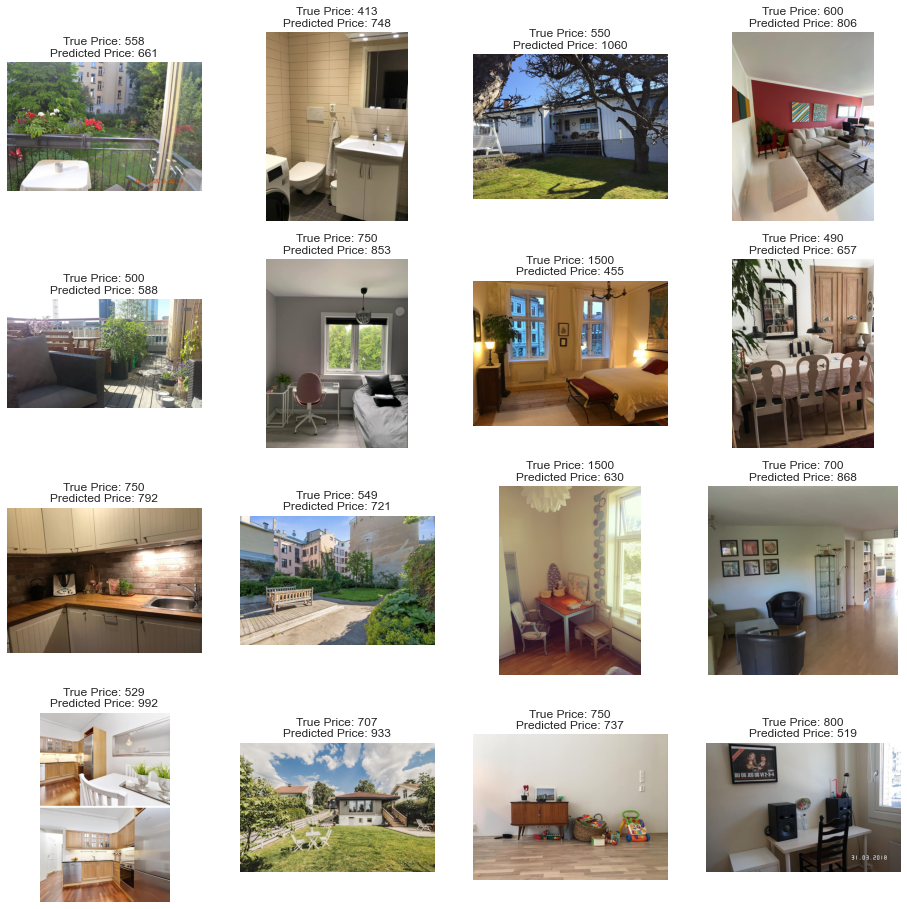
\includegraphics[width=\textwidth]{cnn_examples.png}
    \caption{Images from Airbnb Apartments with true and predicted Prices}
    \label{fig:cnn-examples}
\end{figure}
%%%

\end{document}